\chapter{Experiment}

The experiment was conducted on the ROS bag taken during the first rehearsal attempt. The robot drove around the perimeter to map the whole arena using the Gmapping package. The brick pattern is placed in the left bottom quadrant and the drone delivery in the right top quadrant of the arena.

 It was surprising that the organizers chose the arena with a significant slope in the middle. We did not expect perfectly flat ground, but the angle of the slope was much higher than our expectations. Besides, the middle part of the arena was made of different - very smooth surface, which negatively influenced odometry, especially in rotational movement. That makes the localization in the middle much more difficult because, in this place, the robot is tilted, so the laserscan aims into the ground or into the height, and there is also a quite high distance to the nearest significant feature inside the map, which could help to adjust the position. This behavior is visible on the particle cloud during the experiment. When the robot arrives in the middle, the particles are spread into the width. These circumstances caused many problems to teams, which trained for the contest in laboratory grade conditions. Also, it is necessary to mention that there were many people inside the arena during our experiment, which makes the detection even more challenging because people could be easily interpreted as a red pile. Visualization of experiment is shown in the Figure \ref{fig:experiment}.

The robot managed to localize all interest points even though the line segmentation produces a large number of false-positive detections. A significant advantage for the detection is that the clusters are merging measurements from different positions and because the robot is moving during the detections, it is improbable to accumulate multiple false positive detections into the one cluster. Thus these false-positive candidates have very low confidence, and it is not hard for the EM algorithm to find the actual position of interest points. 

At the beginning of ROS bag the robot drives around the piles in approximate distance of 5m and then in approximate distance of 4m to UAV destination wall. At the end the robot drives back to the center of map and comes closer to the red pile. For experiment was used detection pipeline as desribed in Figure \ref{fig:flowchart}. Value of all constants is listed in Table \ref{tab:constants}. We conducted additional experiments when we tested only individual parts of the detection pipeline. In following sections are measured the precision of such a detections.


\begin{figure}[H]
	\centering
	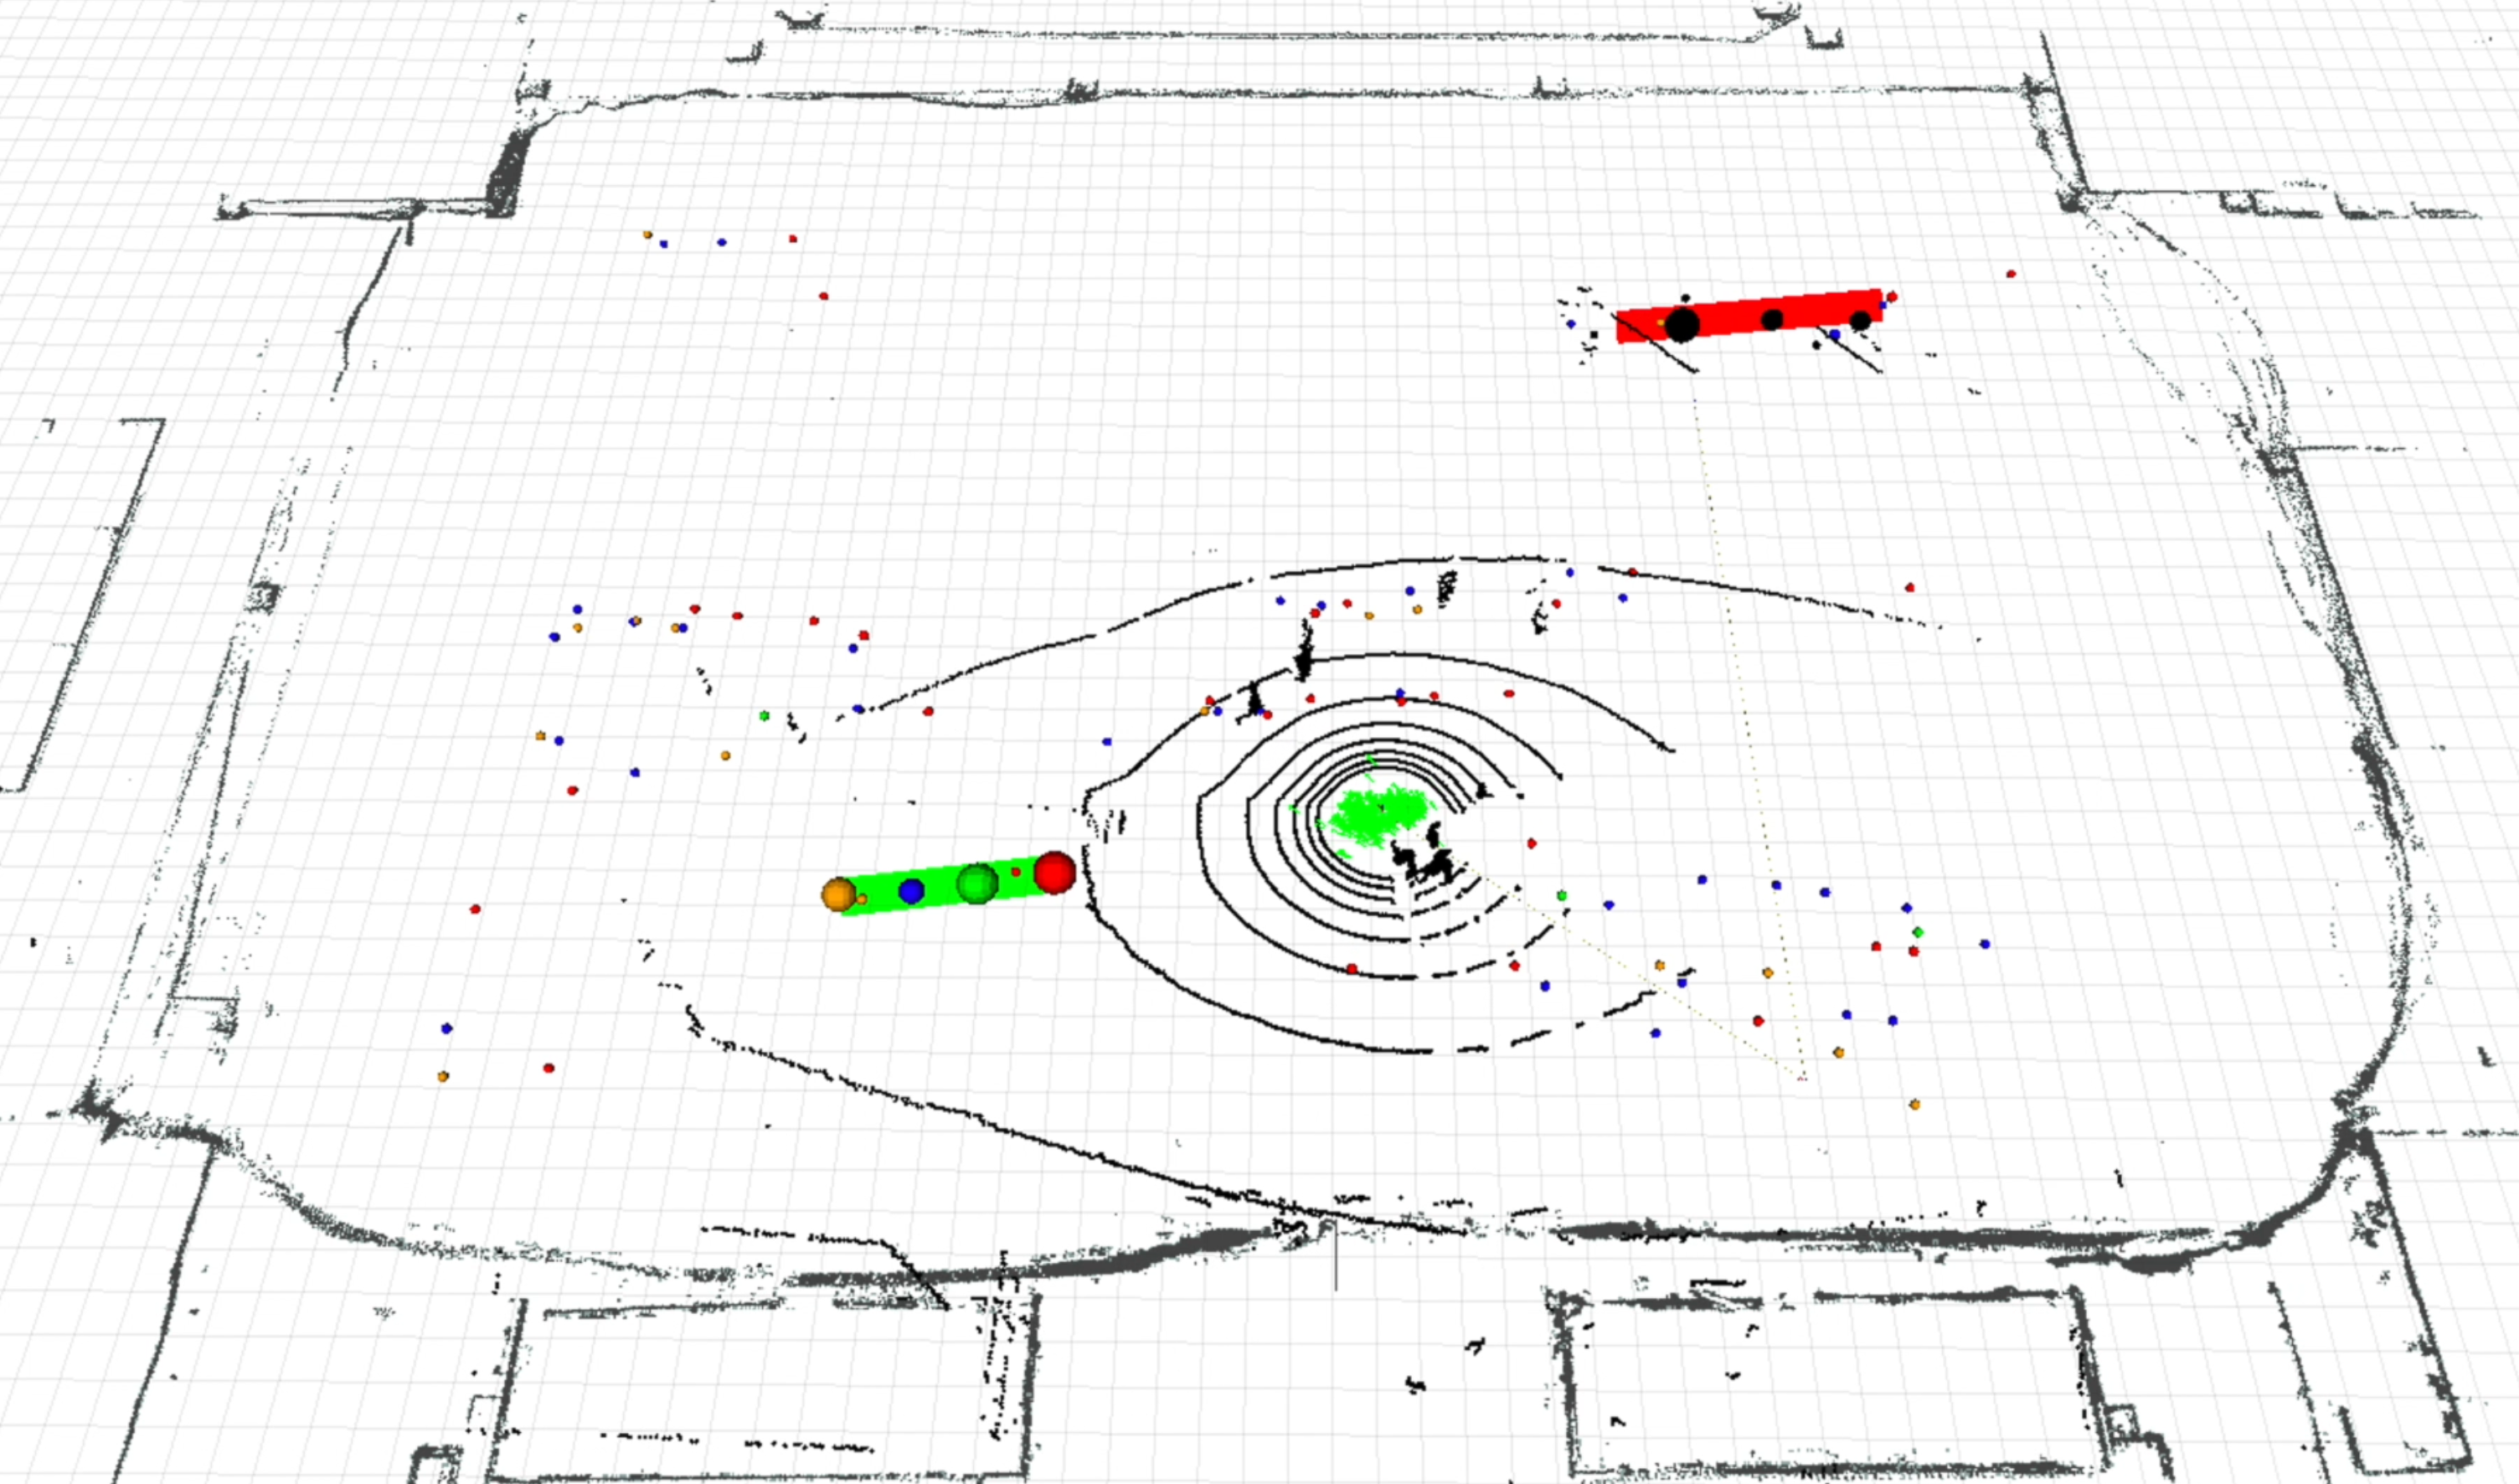
\includegraphics[scale=0.3]{fig/experiment}
	\caption[Experiment results]{In the figure is a screenshot from the experiment \footnotemark. Small spheres on the map are polled clusters from the symbolic map. Different types of detections create these clusters. The size of the sphere represents the confidence of a cluster. The spheres' color corresponds to the color of bricks, and the spheres representing the clusters for UAV destination are colored black. Black is also the pointcloud obtained from lidar and borders of the map. In green color are visualized all particles from the AMCL and also the line representing detection of initial brick pattern. A red line marks the position and rotation of the UAV destination. Note that the RANSAC detector was disabled in this experiment to test the EM algorithm fitting properly.}
	\label{fig:experiment}
\end{figure}
\footnotetext{\url{https://www.youtube.com/watch?v=KKpCGdJnv7Y} } 

\begin{table}[H]
	\centering
	\begin{tabular}{cc}
		\toprule
		Constant & Value \\
		\midrule
		$C$ [m] & 0.07   \\ 
		$S$ [m] & 0.07  \\
		$\sigma_x$ [m] & 0.3 \\ 
		$\sigma_y$ [m] & 0.3 \\
		$d_{inlier}$ [m] & 0.05 \\ 
		$min\_size$ & 10 \\
		$max\_err$ [m] & 0.04 \\
		$cluster\_size$ [m] & 0.5 \\
		$\vec{k}_{pile} $ [m] & $\begin{bmatrix}
			-2.9 & -1 & 0.75 & 2.75
		\end{bmatrix}$ \\
		$\vec{k}_{destination}$ [m] &
		$\begin{bmatrix}
			-\cfrac{6}{\sqrt{2}} &  -\cfrac{2}{\sqrt{2}} &  \cfrac{2}{\sqrt{2}} &  \cfrac{6}{\sqrt{2}}
		\end{bmatrix}$ \\
		\bottomrule
	\end{tabular}
	\caption{List of constants used in experiment.}
	\label{tab:constants}
\end{table}

\section{Precision of detections}
Although all the objects of interest were correctly localized, it is visible in the Table \ref{tab:seg_precision} that the line segmentation produces high number of false positive candidates. That is caused mainly by incorrect filtering of ground plane. This behavior is further discussed in the next section. Very advantageous is that the EM algorithm converges well, until the correct clusters has at least slightly higher confidence than the false positives. It is no surprise that the most frequently detected brick is the red one, because it is the smallest of bricks and there is higher number of red bricks than bricks of any other color. Similarly the blue bricks are the rarest in the arena and blue pile is also the hardest one to detect as shown in the Table \ref{tab:pile_precision}. The UAV destination wall has so low number of false positive detections mainly because the filtered segment has size of $4$m, which is much larger segment than any brick. It is unlikely to obtain such a large false positive segment in relatively empty arena.

The pile detector is very reliable which confirms that the conditions described in section \ref{sec:pile_detector} were chosen correctly. Both false positive detections were probably caused by pedestrians inside the arena. Finally the RANSAC detector produced zero false positives detections, that is mainly thanks to our very strict conditions to even start RANSAC fitting and also thanks to very low inlier distance. This level of precision is achieved mainly because we prefer precision over the detection range, which is the lowest of all detectors. In the experiment the robot drove much closer to the pile from behind, so in the Table \ref{tab:RANSAC_precision} is visible that the rear model was applied more times. It is noteworthy that the EM algorithm was able to fit the hypothesis correctly even when only the individual detection methods were used.

\begin{table}[H]
	\centering
	\begin{tabular}{ccccccc}
		\toprule
		Type &\quad& True &\quad& False &\quad& Precision \\
		\midrule
		Red &\quad& 174 &\quad& 70 &\quad&71.3\% \\
		Green &\quad& 57 &\quad& 19 &\quad& 75\% \\
		Blue &\quad& 24 &\quad& 63 &\quad& 27.5\% \\
		Orange &\quad& 32 &\quad& 20 &\quad& 61.5\% \\
		Wall &\quad& 280 &\quad& 11 &\quad& 96.2\% \\
		\bottomrule
	\end{tabular}
	\caption{Precision of line segmentation.}
	\label{tab:seg_precision}
\end{table}


\begin{table}[H]
	\centering
	\begin{tabular}{ccccccc}
		\toprule
		Type &\quad& True &\quad& False &\quad& Precision \\
		\midrule
		Red &\quad& 39 &\quad& 1 &\quad& 97.5\% \\
		Green &\quad& 36 &\quad& 0 &\quad& 100\% \\
		Blue &\quad& 14 &\quad& 1 &\quad& 93.3\% \\
		Orange &\quad& 17 &\quad& 0 &\quad& 100\% \\
		\bottomrule
	\end{tabular}
	\caption{Precision of pile detection.}
	\label{tab:pile_precision}
\end{table}


\begin{table}[H]
	\centering
	\begin{tabular}{ccccccc}
		\toprule
		Type &\quad& True &\quad& False &\quad& Precision \\
		\midrule
		Front model &\quad& 1 &\quad& 0 &\quad& 100\% \\
		Rear model &\quad& 9 &\quad& 0 &\quad& 100\% \\
		\bottomrule
	\end{tabular}
	\caption{Precision of RANSAC detector.}
	\label{tab:RANSAC_precision}
\end{table}


\section{Ground Segmentation}
As we already mentioned, the ground segmentation applied in this experiment was not sufficient enough. The slope inside the area was responsible for a high number of false-positive detections. The easiest possible ground segmentation method was used in the detector because we did not expect such harsh terrain. The height of lidar above the ground was $0.45$m, so all points with $z$ coordinate lower than $-0.4$m were filtered out of the measurement. This method can segment only wholly flat ground, which was not the case of the arena.

Ground segmentation is a popular subject of study. There are various published papers concerning this topic. Some methods are incorporating machine learning \cite{velas2018}. The usage of machine learning again involves evaluating neural networks, and that can be inefficient on CPU. There are also purely algorithmic methods that perform well even in rough terrain \cite{phuong2019}. These methods do not incorporate any knowledge about the environment, which is not entirely our case, because the arena terrain is known in advance.

We had available advanced mapping device (Leica BLK 360), which is able to create a model of the arena using very dense pointcloud. Such a pointcloud can then be used to create an elevation map of the arena. This elevation map can help to segment out the ground in the robot measurements. Firstly it would be necessary to implement queries to such a map. Then the robot could obtain the transformation of pointcloud using its position. When the candidates are generated, it could be verified whether the candidate is above the terrain. This method would work reasonably well until the localization of the robot works fine.

\section{Time benchmark}
The execution time of each detection algorithm is highly dependent on input size. The line segmentation time complexity grows quadratically with the number of samples \cite{hershberger2000}. It is the most time-consuming part of the whole pipeline because, unlike the pattern fitting, it must be done each iteration. The time complexity of the pile detector (EM algorithm) and the RANSAC algorithm is linear, but both methods usually have a low number of inputs, so the final execution time is very short. 

On the other hand, Pattern fitting is also using the EM algorithm, but it polls the whole history of detections from the symbolic map. Hence it has a much higher number of inputs, and it takes a long time. In our implementation was the pattern fitting ran on every received pointcloud, but that is not necessary because the whole method is deterministic, and the results are different only after a significant change in the symbolic map. Relative lengths of execution is visualized in the Figure \ref{fig:time}. We have compared the measured execution time to lidar frequency, and the detector frequency is significantly lower than the sensor's frequency, so the detection pipeline is not a limiting factor for the robot.

\begin{figure}[H]
	\centering
	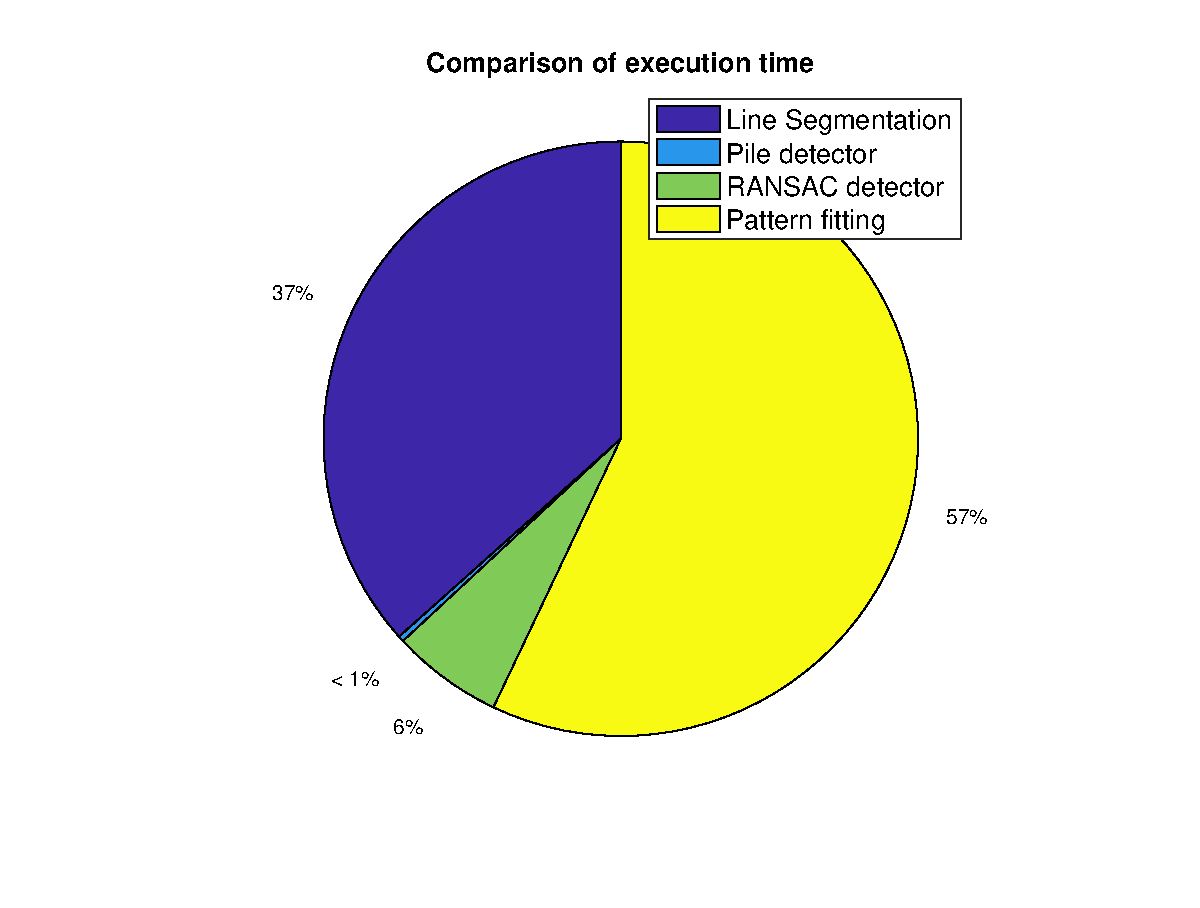
\includegraphics[scale=0.55]{fig/time.eps}
	\caption[Experiment results]{Relative comparison of mean execution time. Whole detection pipeline took on average $4.3$ms (CPU Intel i7 7700k).}
	\label{fig:time}
\end{figure}

